\documentclass[a4paper]{article}
\usepackage{amsmath,amsfonts,amsthm,amssymb}
\usepackage{graphicx}

\title{trivial}
\author{\(\mathbb G\mathbf O\mathbb N \mathbf D\mathbb O\mathbf N\)}
\date{42/0/69}

\begin{document}
\maketitle
\section*{a)}
\begin{enumerate}
    \item The row of `number of students' is above the row of `number of hours spent'.
    \item The columns of 'number of hours spent' are not in order.
\end{enumerate}

\section*{b)}
\subsection*{i)}
\[\begin{aligned}
    X+515-X+480+138+Y&=1363\\
    Y+1133&=1363\\
    Y&=\boxed{230}
\end{aligned}\]

\subsection*{ii)}
It is given that \(X\geqslant Y\iff X_{\min}=230\).
Also, since the modal number of students is 480, all the other columns must have a number of
students that is smaller than 480. Thus,
\[X_{\max}=479\]
Therefore,
\[\boxed{230\leqslant X\leqslant479}\]

\section*{c)}
\subsection*{i)}
Since the total number of 1363 is odd, the median is represented by one student. Hence, the number of hours corresponding the 138 students must be 4. The median position is \((1363+1)/2=682\).
For the median number of hours spent to be 4, there are two requirements for \(X\):
\[\begin{cases}
    230+X_{\min}+138=682\\
    230+X_{\max}+1=682
\end{cases}
\iff
\begin{cases}
    X_{\min}=314\\
    X_{\max}=451
\end{cases}\]
Therefore,
\[\boxed{314\leqslant X\leqslant451}\]

\subsection*{ii)}
\(X\) from (ci) is valid, because \(([314,451]\cup\mathbb N)\subseteq([230,479]\cup\mathbb N)\).


\section*{d)}
\subsection*{i)}
\[{\bar x}_{\min}=\frac{3(451)+5(515-451)+6(480)+4(138)+2(230)}{1363}=\boxed{\frac{5565}{1363}}\]
\[{\bar x}_{\max}=\frac{3(314)+5(515-314)+6(480)+4(138)+2(230)}{1363}=\boxed{\frac{5839}{1363}}\]

\subsection*{ii)}
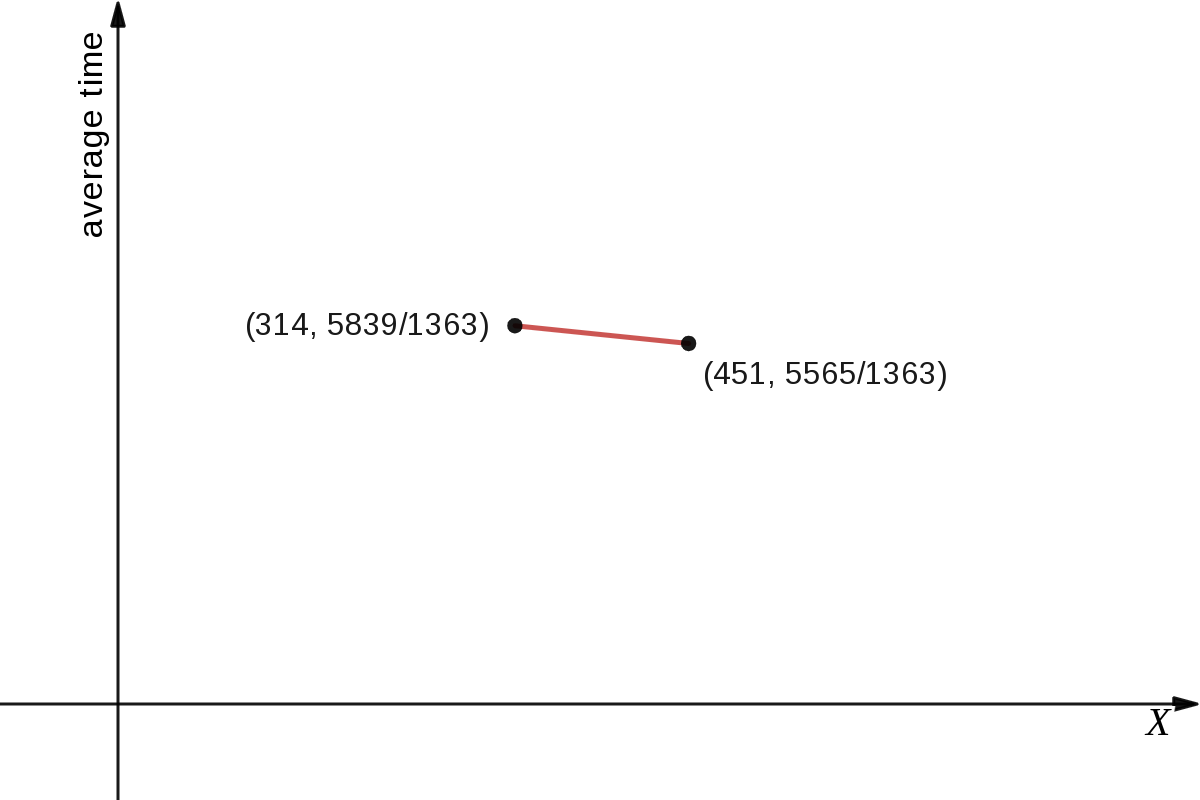
\includegraphics[width=\textwidth]{trivial.png.png}

\section*{e)}
\[\begin{array}{|l|c|c|c|c|c|}
    \hline
    \text{Number of hours spent}&2&3&4&5&6\\
    \hline
    \text{Number of students}&230&455&138&60&480\\
    \hline
\end{array}\]

\section*{f)}
\subsection*{i)}
Mode is equal to 6 hours because 480 is still the largest number of students amongst all the columns. From the extrapolation of the graph in (dii), the median is smaller than 4 hours because
\(X=455\) correspond to the right-hand side portion of the graph, which shows a lower
average time, hence a lower median.
\subsection*{ii)}
\[\text{mean}=\frac{2(230)+3(455)+4(138)+5(60)+6(480)}{1363}=\boxed{\frac{5557}{1363}}\]
\[\text{median}=\boxed3\]
\[\text{mode}=\boxed6\]
\end{document}
